\documentclass[tikz,border=8pt]{standalone}
% Shared look for every TikZ diagram. Load with \input{../../tools/tikz-style.tex}
\usepackage[T1]{fontenc}
\usepackage{lmodern}
\renewcommand{\sfdefault}{lmr}  % diagrams use the same serif as the text
\usetikzlibrary{arrows.meta, positioning, shapes.geometric, calc, fit, backgrounds}
\definecolor{cblue}{HTML}{4C78A8}
\definecolor{corange}{HTML}{F58518}
\definecolor{cgreen}{HTML}{54A24B}
\definecolor{cred}{HTML}{E45756}
\definecolor{cpurple}{HTML}{B279A2}
\definecolor{cgrey}{HTML}{6B6B6B}
\tikzset{
  every picture/.style={font=\sffamily, line width=1.2pt},
  box/.style={draw=#1, fill=#1!12, rounded corners=4pt, align=center, inner sep=7pt, minimum height=1.1cm},
  box/.default=cgrey,
  arrow/.style={-{Stealth[length=3mm]}, draw=cgrey, line width=1.4pt},
  title/.style={font=\sffamily\bfseries\Large},
  note/.style={font=\sffamily\small, text=cgrey, align=center},
}
\AtBeginDocument{\hyphenpenalty=10000 \exhyphenpenalty=10000}

% Prediction step at t = 2 (command: push) as a probability tree. The door was open (0.75) or closed (0.25); a push
% keeps an open door open (1) and opens a closed door with 0.8. The two paths that end "open" add to 0.95.
\begin{document}
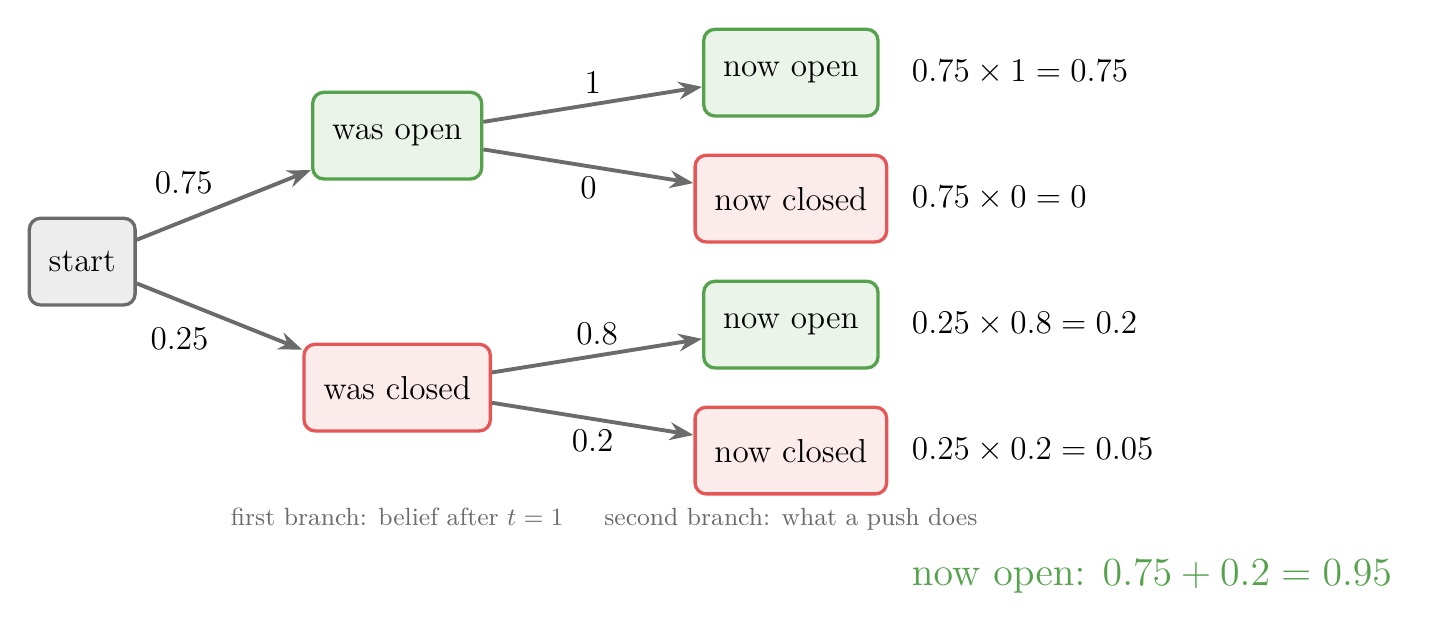
\begin{tikzpicture}[x=1cm, y=1cm, every node/.append style={font=\large}]
  \node[box] (s) at (0,0) {start};
  \node[box=cgreen] (o) at (4,1.6) {was open};
  \node[box=cred] (c) at (4,-1.6) {was closed};
  \draw[arrow] (s) -- node[above left] {0.75} (o);
  \draw[arrow] (s) -- node[below left] {0.25} (c);
  \node[box=cgreen] (oo) at (9,2.4) {now open};
  \node[box=cred] (oc) at (9,0.8) {now closed};
  \node[box=cgreen] (co) at (9,-0.8) {now open};
  \node[box=cred] (cc) at (9,-2.4) {now closed};
  \draw[arrow] (o) -- node[above] {1} (oo);
  \draw[arrow] (o) -- node[below] {0} (oc);
  \draw[arrow] (c) -- node[above] {0.8} (co);
  \draw[arrow] (c) -- node[below] {0.2} (cc);
  \node[anchor=west] at (10.4,2.4) {$0.75 \times 1 = 0.75$};
  \node[anchor=west] at (10.4,0.8) {$0.75 \times 0 = 0$};
  \node[anchor=west] at (10.4,-0.8) {$0.25 \times 0.8 = 0.2$};
  \node[anchor=west] at (10.4,-2.4) {$0.25 \times 0.2 = 0.05$};
  \node[note, anchor=north] at (4,-3.0) {first branch: belief after $t = 1$};
  \node[note, anchor=north] at (9,-3.0) {second branch: what a push does};
  \node[anchor=west, cgreen, font=\Large] at (10.4,-4.0) {now open: $0.75 + 0.2 = 0.95$};
\end{tikzpicture}
\end{document}
